% !TeX root = ../main.tex

\section* {Dirichlet Process}

The Dirichlet Process to model infinite gaussian mixtures.

\paragraph{Short reminder: Gaussian mixture models}
\begin{enumerate}
    \item What is a GMM? \(\Rightarrow \sum_{i=1}^k \beta_i \mathcal{N}(\mu_i, \Sigma_i)\)
    \item What parameters? \(\Rightarrow \beta_i, \mu_i, \Sigma_i\)
    \item How do I determine these parameters? \(\Rightarrow EM-Algorithm\)

          Start with random initialization, expectation (how much does each component contribute to each point), maximization (update component parameters), repeat until convergence

          From a more abstract perspective, EM performs two tasks simultaneously: segmentation/clustering assignment, and model parameters estimation/fitting
\end{enumerate}

\paragraph{The idea for infinite mixture models:}
Instead of fitting a specific distribution to the data (the GMM), we define a meta-distribution from which the actual distribution is drawn.
specifically we can draw a GMM from a dirichlet process\footnote{Because uniform ??? parameters for drawing the GMM}. However this is a top-down perspective, i.e. if we randomly draw a GMM, we will certainly not draw one that fits nicely to our data.
From a bottom up perspective, we need a fitting algorithm that works with the available data points and finds a GMM in such a way, that it could also have been drawn from a distribution of distributions (the dirichlet process).
To illustrate the model behind the fitting algorithm, we usually talk about the ``\textbf{Chinese restaurant process}'' (CRP).

\begin{figure}[H]
	\centering
	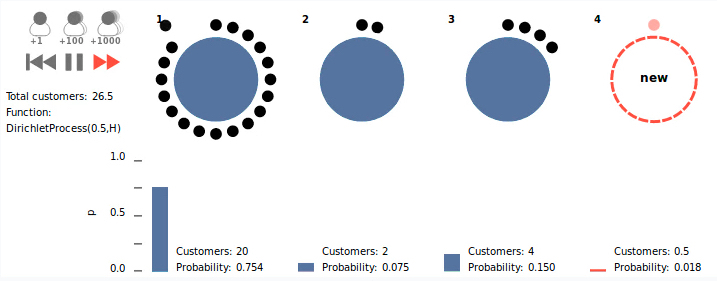
\includegraphics[width=0.6\textwidth]{chinese_restaurant_process}
  \caption{There are tables in a restaurant (our mixture components). Whenever a new customer comes in (a sample), it chooses the table it most relates to. When the customer is unsatisfied with current offering, he can open up a new table (\href{https://en.wikipedia.org/wiki/Chinese_restaurant_process}{Check the explaination form wikipedia}).}
\end{figure}

\paragraph{Extensions to a ``normal'' GMM:}
\begin{enumerate}
	\item If a customer prefers to sit at a new table, this is possible we can add arbitrary many tables
	\item The more people sit on a table  the more attractive it is to the new customers (rich get richer)
\end{enumerate}

The chinese restaurant process (CRP) provides a constructive way of sampling from a dirichlet process.

\paragraph{Gibbs sampling:}
A straight forward (probailistic\footnote{because we sample from the list ..???}) clustering algorithm based on the CRP

\begin{enumerate}
    \item Init: assign each sample to a cluster (e.g. randomly, or do \(k-\)means)
    \item Randomly select a sample \(x_i\) from the data
    \item Compute a affinity of \(x_i\) to each table: \(t_i = \frac{N_i}{N+\alpha} \mathcal{N}(x_i, \mu_i, \Sigma_i)\) (Gaussian distance of \(x_i\) to \(\mathcal(\mu_i, \Sigma_i)\)), where \(N_i\) is the number of customers on the table (number of samples assigned to \(\mathcal{N}(\mu_i, \Sigma_i)\) and \(N\) is the total number of samples, \(\alpha\) is an "expansion parameter"
    \item Compute affinity to a new table \(t_0 = \frac{\alpha}{N + \alpha} \cdot \mathcal{N}(x_i, \mu_0, \Sigma_0)\)
    \item Collect all affinities \(t_0, \dots, t_T\) in a list, normalize sum to one
    \item Sample from that list a table assignment (all affinities are interpreted as a PDF from which we sample)
    \item Recompute \(\mu_i, \Sigma_i\) for the assigned table
    \item Goto 2, stop after certain number of iterations
\end{enumerate}

\paragraph{Back to the top-down view:}
Using the CRP, we are effectivly drawing a GMM using a dirichlet process. Implicitly, the mixture weihts $\beta_i$ match a $Beta(\alpha)$ distribution and the normal distributions are drawn from a hyper-distribution, i.e. $\vartheta_i \sim H(\lambda)$

\paragraph{Stick breaking process:} \href{https://en.wikipedia.org/wiki/Dirichlet_process#The_stick-breaking_process}{(check the wiki-page)}
\begin{figure}[H]
  \centering
  \begin{minipage}[b]{0.49\textwidth}
    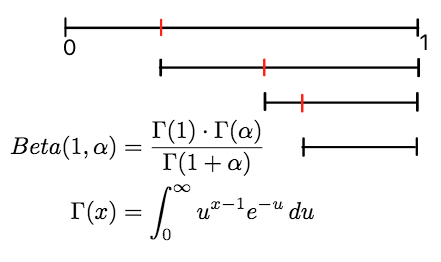
\includegraphics[width=\textwidth]{stick_breaking_process}
    \caption{Illustration of a $Beta$ distribution}
  \end{minipage}
  \begin{minipage}[b]{0.49\textwidth}
    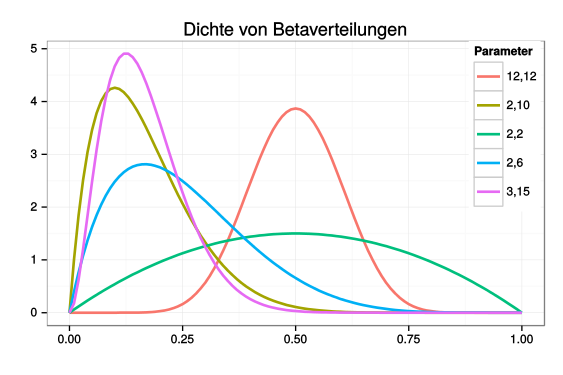
\includegraphics[width=\textwidth]{Beta_distribution}
    \caption{Qualitatively, this is what the $Beta$ distribution looks like}
  \end{minipage}
\end{figure}

The expansion parameter $\alpha$ is a prior that influences the number of clusters that will be created.

\paragraph{Observation 1:}
The larger the expansion parameter $\alpha$ is, the more likely it is to draw a number that is close to $0$ form $Beta(1,\alpha)$

The number that has been drawn form $Beta(1,\alpha)$ is used in the stick breaking process to determine the weight of the i-th mixture component $\beta_i$

\paragraph{Observation 2:}
The number that has been drawn from \(Beta(1,\alpha)\) is used in the stick breaking process to determine the weight of the \(i\)-th mixture component \(\beta_i\).

\paragraph{Stick breaking process (formalised):}

\begin{equation*}
	b_i \sim Beta(1,\alpha)
\end{equation*}

\begin{equation*}
	\beta_i = b_i \dot \prod_{i=1}^{i-1}(1-b_i) = b_i (1 - \sum_{i=1}^{i-1} \beta_i)
\end{equation*}

% TODO ask moe for the missing picture
% \begin{figure}[H]
% 	\centering
% 	
\includegraphics[width=0.5\textwidth]{todo}
% \end{figure}
